% \documentclass[a4paper,dvipsnames]{article}

% \addtolength{\hoffset}{-2.25cm}
% \addtolength{\textwidth}{4.5cm}
% \addtolength{\voffset}{-3.25cm}
% \addtolength{\textheight}{5cm}
% \setlength{\parskip}{0pt}
% \setlength{\parindent}{0in}

% %----------------------------------------------------------------------------------------
%	PACKAGES AND OTHER DOCUMENT CONFIGURATIONS
%----------------------------------------------------------------------------------------

%----------------------------------------------------------------------------------------
%		Generals
%----------------------------------------------------------------------------------------
\usepackage{fourier}
\usepackage{frcursive}
\usepackage[T1]{fontenc} %Accents handling
\usepackage[utf8]{inputenc} % Use UTF-8 encoding
%\usepackage{microtype} % Slightly tweak font spacing for aesthetics
\usepackage[english, francais]{babel} % Language hyphenation and typographical rules

%----------------------------------------------------------------------------------------
%		Graphics
%----------------------------------------------------------------------------------------
\usepackage{xcolor}
\usepackage{graphicx, multicol} % Enhanced support for graphics
\graphicspath{{FIG/}}
\usepackage{wrapfig}

%----------------------------------------------------------------------------------------
%		Other packages
%----------------------------------------------------------------------------------------
\usepackage{hyperref}
\hypersetup{
	colorlinks=true, %colorise les liens
	breaklinks=true, %permet le retour à la ligne dans les liens trop longs
	urlcolor= bleu3,  %couleur des hyperliens
	linkcolor= bleu3, %couleur des liens internes
	plainpages=false  %pour palier à "Bookmark problems can occur when you have duplicate page numbers, for example, if you have a page i and a page 1."
}
\usepackage{tabularx}
\newcolumntype{M}[1]{>{\arraybackslash}m{#1}} %Defines a scalable column type in tabular
\usepackage{booktabs} % Enhances quality of tables
\usepackage{diagbox} % barre en diagonale dans un tableau
\usepackage{multicol}
\usepackage[explicit]{titlesec}


%----------------------------------------------------------------------------------------
%		Headers and footers
%----------------------------------------------------------------------------------------
\usepackage{fancyhdr} % Headers and footers
\pagestyle{fancy} % All pages have headers and footers
\fancyhead{}\renewcommand{\headrulewidth}{0pt} % Blank out the default header
\renewcommand{\footrulewidth}{0pt}
\fancyfoot[L]{} % Custom footer text
\fancyfoot[C]{\href{https://sacado.xyz/}{sacado.xyz}} % Custom footer text
\fancyfoot[R]{\thepage} % Custom footer text

%----------------------------------------------------------------------------------------
%		Mathematics packages
%----------------------------------------------------------------------------------------
\usepackage{amsthm, amsmath, amssymb} % Mathematical typesetting
\usepackage{marvosym, wasysym} % More symbols
\usepackage[makeroom]{cancel}
\usepackage{xlop}
\usepackage{pgf,tikz,pgfplots}
\pgfplotsset{compat=1.15}
\usetikzlibrary{positioning}
%\usetikzlibrary{arrows}
\usepackage{pst-plot,pst-tree,pst-func, pstricks-add,pst-node,pst-text}
\usepackage{units}
\usepackage{nicefrac}
\usepackage[np]{numprint} %Séparation milliers dans un nombre

%----------------------------------------------------------------------------------------
%		New text commands
%----------------------------------------------------------------------------------------
\usepackage{calc}
\usepackage{boites}
 \renewcommand{\arraystretch}{1.6}

%%%%% Pour les imports.
\usepackage{import}

%%%%% Pour faire des boites
\usepackage[tikz]{bclogo}
\usepackage{bclogo}
\usepackage{framed}
\usepackage[skins]{tcolorbox}
\tcbuselibrary{breakable}
\tcbuselibrary{skins}
\usetikzlibrary{babel,arrows,shadows,decorations.pathmorphing,decorations.markings,patterns}

%%%%% Pour les symboles et les ensembles
\newcommand{\pp}{\leq}
\newcommand{\pg}{\geq}
%\newcommand{\euro}{\eurologo{}}
\newcommand{\R}{\mathbb{R}}
\newcommand{\N}{\mathbb{N}}
\newcommand{\D}{\mathbb{D}}
\newcommand{\Z}{\mathbb{Z}}
\newcommand{\Q}{\mathbb{Q}}
\newcommand{\C}{\mathbb{C}}

%%%%% Pour une double minipage
\newcommand{\mini}[2]{
\begin{minipage}[t]{0.48\linewidth}
#1
\end{minipage}
\hfill
\begin{minipage}[t]{0.48\linewidth}
#2
\end{minipage}
}


%\newcommand\hole[1]{\texttt{\_}}
%\newcommand{\PROP}[1]{\textbf{\underline{#1}}}
%\newcommand{\exercice}{\textcolor{OliveGreen}{Exercice : }}
%\newcommand{\correction}{\textcolor{BurntOrange}{Correction : }}
%\newcommand{\propriete}{\textbf{\underline{Propriété}} : }
%\newcommand{\prop}{\textbf{\underline{Propriété}} : }
%\newcommand{\vocabulaire}{\textbf{\underline{Vocabulaire}} : }
%\newcommand{\voca}{\textbf{\underline{Vocabulaire}} : }

\usepackage{enumitem}
\newlist{todolist}{itemize}{2} %Pour faire des QCM
\setlist[todolist]{label=$\square$} %Pour faire des QCM \begin{todolist} instead of itemize

%----------------------------------------------------------------------------------------
%		Définition de couleur pour geogebra
%----------------------------------------------------------------------------------------
\definecolor{zzttqq}{rgb}{0.6,0.2,0.} %rouge des polygones
\definecolor{qqqqff}{rgb}{0.,0.,1.}
\definecolor{xdxdff}{rgb}{0.49019607843137253,0.49019607843137253,1.}%bleu
\definecolor{qqwuqq}{rgb}{0.,0.39215686274509803,0.} %vert des angles
\definecolor{ffqqqq}{rgb}{1.,0.,0.} %rouge vif
\definecolor{uuuuuu}{rgb}{0.26666666666666666,0.26666666666666666,0.26666666666666666}
\definecolor{qqzzqq}{rgb}{0.,0.6,0.}
\definecolor{cqcqcq}{rgb}{0.7529411764705882,0.7529411764705882,0.7529411764705882} %gris
\definecolor{qqffqq}{rgb}{0.,1.,0.}
\definecolor{ffdxqq}{rgb}{1.,0.8431372549019608,0.}
\definecolor{ffffff}{rgb}{1.,1.,1.}
\definecolor{ududff}{rgb}{0.30196078431372547,0.30196078431372547,1.}

%-------------------------------------------------
%
%	EN TETE
%
%-------------------------------------------------

% Classe
\newcommand{\myClasse}   
{
    6e
}

% Discipline
\newcommand{\myDiscipline}   
{
    Mathématiques
}

% Parcours
\newcommand{\myParcours}
{
  Nombres et Calculs
}

%Titre de la séquence
\newcommand{\myTitle}
{
    \scshape\huge
\textcolor{sacado_purple}{
		Nombres décimaux
}
}

%----------------------------------------------------------------------------------------

% %----------------------------------------------------------------------------------------
%		Définition de couleur pour les boites
%----------------------------------------------------------------------------------------
\definecolor{bleu1}{rgb}{0.54,0.79,0.95} %% Bleu
\definecolor{sapgreen}{rgb}{0.4, 0.49, 0}
\definecolor{dvzfxr}{rgb}{0.7,0.4,0.}
\definecolor{beamer}{rgb}{0.5176470588235295,0.49019607843137253,0.32941176470588235} % couleur beamer
\definecolor{preuveRbeamer}{rgb}{0.8,0.4,0}
\definecolor{sectioncolor}{rgb}{0.24,0.21,0.44}
\definecolor{subsectioncolor}{rgb}{0.1,0.21,0.61}
\definecolor{subsubsectioncolor}{rgb}{0.1,0.21,0.61}
\definecolor{info}{rgb}{0.82,0.62,0}
\definecolor{bleu2}{rgb}{0.38,0.56,0.68}
\definecolor{bleu3}{rgb}{0.24,0.34,0.40}
\definecolor{bleu4}{rgb}{0.12,0.20,0.25}
\definecolor{vert}{rgb}{0.21,0.33,0}
\definecolor{vertS}{rgb}{0.05,0.6,0.42}
\definecolor{red}{rgb}{0.78,0,0}
\definecolor{color5}{rgb}{0,0.4,0.58}
\definecolor{eduscol4B}{rgb}{0.19,0.53,0.64}
\definecolor{eduscol4P}{rgb}{0.62,0.12,0.39}

%----------------------------------------------------------------------------------------
%		Définition de couleur pour les boites SACADO
%----------------------------------------------------------------------------------------
\definecolor{sacado_blue}{RGB}{0,129,159} %% Bleu Sacado
\definecolor{sacado_green}{RGB}{59, 157, 38} %% Vert Sacado
\definecolor{sacado_yellow}{RGB}{255,180,0} %% Jaune Sacado
\definecolor{sacado_purple}{RGB}{94,68,145} %% Violet foncé Sacado
\definecolor{sacado_violet}{RGB}{153,117,224} %% Violet clair Sacado
\definecolor{sacado_orange}{RGB}{249,168,100} %% Orange Sacado
\definecolor{ill_frame}{HTML}{F0F0F0}
\definecolor{ill_back}{HTML}{F7F7F7}
\definecolor{ill_title}{HTML}{AAAAAA}


 % Compteurs pour Théorème, Définition, Exemple, Remarque, .....
\newcounter{cpttheo}
\setcounter{cpttheo}{0}
\newcounter{cptdef}
\setcounter{cptdef}{0}
\newcounter{cptmth}
\setcounter{cptmth}{0}
\newcounter{cpttitre}
\setcounter{cpttitre}{0}
 % Exercices
\newcounter{cptapp}
\setcounter{cptapp}{0}
\newcounter{cptex}
\setcounter{cptex}{0}
\newcounter{cptsr}
\setcounter{cptsr}{0}
\newcounter{cpti}
\setcounter{cpti}{0}
\newcounter{cptcor}
\setcounter{cptcor}{0}




%%%%% Pour réinitialiser numéros des paragraphes après une nouvelle partie
\makeatletter
    \@addtoreset{paragraph}{part}
\makeatother


%%%% Titres et sections

\newlength\chapnumb
\setlength\chapnumb{3cm}


% \titleformat{\part}[block] {
 % \normalfont\sffamily\color{violet}}{}{0pt} {
   % \parbox[t]{\chapnumb}{\fontsize{120}{110}\selectfont\ding{110}}
   % \parbox[b]{\dimexpr\textwidth-\chapnumb\relax}{
       % \raggedleft
       % \hfill{{\color{bleu3}\fontsize{40}{30}\selectfont#1}}\\
       % \rule{0.99\textwidth-\chapnumb\relax}{0.4pt}
 % }
% }

% \titleformat{name=\part,numberless}[block]
% {\normalfont\sffamily\color{bleu3}}{}{0pt}
% {\parbox[b]{\chapnumb}{%
  % \mbox{}}%
 % \parbox[b]{\dimexpr\textwidth-\chapnumb\relax}{%
   % \raggedleft%
   % \hfill{{\color{bleu3}\fontsize{40}{30}\selectfont#1}}\\
   % \rule{0.99\textwidth-\chapnumb\relax}{0.4pt}
 % }
% }



% \titleformat{\chapter}[block] {
 % \normalfont\sffamily\color{violet}}{}{0pt} {
   % \parbox[t]{\chapnumb}{ 
     % \fontsize{120}{110}\selectfont\thechapter}
     % \parbox[b]{\textwidth-\chapnumb}{
       % \raggedleft
       % \hfill{{\color{bleu3}\huge#1}}\\  
  % \ifthenelse{\thechapter<10}{\rule{0.99\textwidth-\chapnumb}{0.4pt}}{\rule{0.9\textwidth - \chapnumb}{0.4pt}}
       % \setcounter{cpttitre}{0}
	% \setcounter{cptapp}{0}
	% \setcounter{cptex}{0}
	% \setcounter{cptsr}{0}
	% \setcounter{cpti}{0}
	% \setcounter{cptcor}{0} 
 % }
% }

% \titleformat{name=\chapter,numberless}[block]
% {\normalfont\sffamily\color{bleu3}}{}{0pt}
% {\parbox[b]{\chapnumb}{%
  % \mbox{}}%
 % \parbox[b]{\textwidth-\chapnumb}{%
   % \raggedleft
   % \hfill{{\color{bleu3}\huge#1}}\\
   % \ifthenelse{\thechapter<10}{\rule{0.99\textwidth-\chapnumb}{0.4pt}}{ \rule{0.9\textwidth - \chapnumb}{0.4pt}}
       % \setcounter{cpttitre}{0}
	% \setcounter{cptapp}{0}
	% \setcounter{cptex}{0}
	% \setcounter{cptsr}{0}
	% \setcounter{cpti}{0}
	% \setcounter{cptcor}{0} 
 % }
% }
%
%       
%
%%%%% Personnalisation des numéros des sections
\renewcommand\thesection{\Roman{section}. }
\renewcommand\thesubsection{\hspace{1cm}\arabic{subsection}. }
\renewcommand\thesubsubsection{\hspace{2cm}\alph{subsubsection}. }

\titleformat{\section}[hang]{\color{sacado_purple}{}\normalfont\filright\huge}{}{0.4em}{\textbf{\thesection  #1}}   
% \titlespacing*{\section}{0.2pt}{0ex plus 0ex minus 0ex}{0.3em}
   
\titleformat{\subsection}[hang]{\color{sacado_purple}{}\normalfont\filright\Large}{}{0.4em}{\thesubsection
 #1}            
\titleformat{\subsubsection}[hang]{\color{sacado_purple}{}\normalfont\filright\large}{}{0.4em}{\thesubsubsection
 #1}
\titleformat{\paragraph}[hang]{\color{black}{}\normalfont\filright\normalsize}{}{0.4em}{#1}



%%%%%%%%%%%%%%%%%%%%% Cycle 4
%\newcommand{\Titre}[2]{\section*{#1 
%\ifthenelse{\equal{#2}{1}}   {\hfill{ \ding{182}  \ding{173} \ding{174} } \addcontentsline{toc}{section}{#1 \ding{182}} }%
%{%
%\ifthenelse{\equal{#2}{2}}{\hfill{ \ding{172}  \ding{183} \ding{174} } \addcontentsline{toc}{section}{#1 {\color{purple}\ding{183}}} }{%           
%\hfill{ \ding{172}  \ding{173} \ding{184} } \addcontentsline{toc}{section}{#1 {\color{orange}\ding{184}}}% 
%}%
%}%
%}
%}


%%%%%%%%%%%%%%%%%%%%% Cycle 4
\newcommand{\Titre}[2]{\section*{#1 
\ifthenelse{\equal{#2}{1}}   {\hfill{ \ding{182}  \ding{173} \ding{174} } \addcontentsline{toc}{section}{#1 \, \ding{182}} }%
{% sinon
\ifthenelse{\equal{#2}{1,5}}   {\hfill{ \ding{182}  \ding{183} \ding{174} } \addcontentsline{toc}{section}{#1 \, \ding{182} {\color{purple}\ding{183}}} }%
{% sinon
\ifthenelse{\equal{#2}{2}}   {\hfill{ \ding{172}  \ding{183} \ding{174} } \addcontentsline{toc}{section}{#1 \, {\color{purple}\ding{183}}} }
{% sinon
\ifthenelse{\equal{#2}{2,5}}   {\hfill{ \ding{172}  \ding{183} \ding{184} } \addcontentsline{toc}{section}{#1 \, {\color{purple}\ding{183}}  {\color{orange}\ding{184}}} }%
{% sinon
\hfill{ \ding{172}  \ding{173} \ding{184} } \addcontentsline{toc}{section}{#1 \,{\color{orange}\ding{184}}}% 
}%
}%
}%
}%
}%
}

%%%%%%%%%%%%% Titre
\newenvironment{titre}[2][]{%
\vspace{0.5cm}
\begin{tcolorbox}[enhanced, lifted shadow={0mm}{0mm}{0mm}{0mm}%
{black!60!white}, attach boxed title to top left={xshift=110mm, yshift*=-3mm}, coltitle=violet, colback=bleu3!25!white, boxed title style={colback=white!100}, colframe=bleu3,title=\stepcounter{cpttitre} \textbf{Fiche \thecpttitre}. #1 #2 ]}
{%
\end{tcolorbox}
\par}



%%%%%%%%%%%%% Définitions
\newenvironment{Def}[1][]{%
\medskip \begin{tcolorbox}[widget,colback=sacado_violet!0,colframe=sacado_violet!75,
adjusted title= \stepcounter{cptdef} Définition \thecptdef . {#1} ]}
{%
\end{tcolorbox}\par}


\newenvironment{DefT}[2][]{%
\medskip \begin{tcolorbox}[widget,colback=sacado_violet!0,colframe=sacado_violet!75,
adjusted title= \stepcounter{cptdef} Définition \thecptdef . {#1} \textit{#2}]}
{%
\end{tcolorbox}\par}

%%%%%%%%%%%%% Proposition
\newenvironment{Prop}[1][]{%
\medskip \begin{tcolorbox}[widget,colback=sacado_blue!0,colframe=sacado_blue!75!black,
adjusted title= \stepcounter{cpttheo} Proposition \thecpttheo . {#1} ]}
{%
\end{tcolorbox}\par}

%%%%%%%%%%%%% Propriétés
\newenvironment{Pp}[1][]{%
\medskip \begin{tcolorbox}[widget,colback=sacado_blue!0,colframe=sacado_blue!75!black,
adjusted title= \stepcounter{cpttheo} Propriété \thecpttheo . {#1}]}
{%
\end{tcolorbox}\par}

\newenvironment{PpT}[2][]{%
\medskip \begin{tcolorbox}[widget,colback=sacado_blue!0,colframe=sacado_blue!75!black,
adjusted title= \stepcounter{cpttheo} Propriété \thecpttheo . {#1} #2]}
{%
\end{tcolorbox}\par}

\newenvironment{Pps}[1][]{%
\medskip \begin{tcolorbox}[widget,colback=sacado_blue!0,colframe=sacado_blue!75!black,
adjusted title= \stepcounter{cpttheo} Propriétés \thecpttheo . {#1}]}
{%
\end{tcolorbox}\par}

%%%%%%%%%%%%% Théorèmes
\newenvironment{ThT}[2][]{% théorème avec titre
\medskip \begin{tcolorbox}[widget,colback=sacado_blue!0,colframe=sacado_blue!75!black,
adjusted title= \stepcounter{cpttheo} Théorème \thecpttheo . {#1} #2]}
{%
\end{tcolorbox}\par}

\newenvironment{Th}[1][]{%
\medskip \begin{tcolorbox}[widget,colback=sacado_blue!0,colframe=sacado_blue!75!black,
adjusted title= \stepcounter{cpttheo} Théorème \thecpttheo . {#1}]}
{%
\end{tcolorbox}\par}

%%%%%%%%%%%%% Règles
\newenvironment{Reg}[1][]{%
\medskip \begin{tcolorbox}[widget,colback=sacado_blue!0,colframe=sacado_blue!75!black,
adjusted title= \stepcounter{cpttheo} Règle \thecpttheo . {#1}]}
{%
\end{tcolorbox}\par}

%%%%%%%%%%%%% REMARQUES
\newenvironment{Rq}[1][]{%
\begin{bclogo}[couleur=sacado_orange!0, arrondi =0.15, noborder=true, couleurBarre=sacado_orange, logo = \bcinfo ]{ 
{\color{info}\normalsize{Remarque#1}}}}
{%
\end{bclogo}
\par}


\newenvironment{Rqs}[1][]{%
\begin{bclogo}[couleur=sacado_orange!0, arrondi =0.15, noborder=true, couleurBarre=sacado_orange, logo = \bcinfo ]{ 
{\color{info}\normalsize{Remarques#1}}}}
{%
\end{bclogo}
\par}

%%%%%%%%%%%%% EXEMPLES
\newenvironment{Ex}[1][]{%
\begin{bclogo}[couleur=sacado_yellow!15, arrondi =0.15, noborder=true, couleurBarre=sacado_yellow, logo = \bclampe ]{ 
\normalsize{Exemple#1}}}
{%
\end{bclogo}
\par}




%%%%%%%%%%%%% Preuve
\newenvironment{Pv}[1][]{%
\begin{tcolorbox}[breakable, enhanced,widget, colback=sacado_blue!10!white,boxrule=0pt,frame hidden,
borderline west={1mm}{0mm}{sacado_blue!75}]
\textbf{Preuve#1 : }}
{%
\end{tcolorbox}
\par}


%%%%%%%%%%%%% PreuveROC
\newenvironment{PvR}[1][]{%
\begin{tcolorbox}[breakable, enhanced,widget, colback=sacado_blue!10!white,boxrule=0pt,frame hidden,
borderline west={1mm}{0mm}{sacado_blue!75}]
\textbf{Preuve (ROC)#1 : }}
{%
\end{tcolorbox}
\par}


%%%%%%%%%%%%% Compétences
\newenvironment{Cps}[1][]{%
\vspace{0.4cm}
\begin{tcolorbox}[enhanced, lifted shadow={0mm}{0mm}{0mm}{0mm}%
{black!60!white}, attach boxed title to top left={xshift=5mm, yshift*=-3mm}, coltitle=white, colback=white, boxed title style={colback=sacado_green!100}, colframe=sacado_green!75!black,title=\textbf{Compétences associées#1}]}
{%
\end{tcolorbox}
\par}

%%%%%%%%%%%%% Compétences Collège
\newenvironment{CpsCol}[1][]{%
\vspace{0.4cm}
\begin{tcolorbox}[breakable, enhanced,widget, colback=white ,boxrule=0pt,frame hidden,
borderline west={2mm}{0mm}{bleu3}]
\textbf{#1}}
{%
\end{tcolorbox}
\par}




%%%%%%%%%%%%% Attendus
\newenvironment{Ats}[1][]{%
\vspace{0.4cm}
\begin{tcolorbox}[enhanced, lifted shadow={0mm}{0mm}{0mm}{0mm}%
{black!60!white}, attach boxed title to top left={xshift=5mm, yshift*=-3mm}, coltitle=white, colback=white, boxed title style={colback=sacado_green!100}, colframe=sacado_green!75!black,title=\textbf{Attendus du chapitre#1}]}
{%
\end{tcolorbox}
\par}

%%%%%%%%%%%%% Méthode
\newenvironment{Mt}[1][]{%
\vspace{0.4cm}
\begin{bclogo}[couleur=sacado_blue!0, arrondi =0.15, noborder=true, couleurBarre=bleu3, logo = \bccrayon ]{ 
\normalsize{{\color{bleu3}Méthode #1}}}}
{%
\end{bclogo}
\par}


%%%%%%%%%%%%% Méthode en vidéo
\newcommand{\MtV}[2]{\vspace{0.4cm} \colorbox{sacado_blue!0}{\hspace{0.2 cm}\tikz\node[rounded corners=1pt,draw] {\color{red}$\blacktriangleright$}; \quad  \href{https://youtu.be/#1?rel=0}{\raisebox{0.8mm}{{\color{red}\textbf{Méthode en vidéo : #2}}}}}}


%%%%%%%%%%%%% A voir (AV) : Lien externe + vidéo non Youtube
\newcommand{\AV}[2]{\vspace{0.4cm} \colorbox{bleu1!0}{\hspace{0.2 cm}\tikz\node[rounded corners=1pt,draw] {\color{red}$\blacktriangleright$}; \quad  \href{#1}{\raisebox{0.8mm}{{\color{red}\textbf{#2}}}}}}


%%%%%%%%%%%%% Etymologie
\newenvironment{Ety}[1][]{%
\begin{bclogo}[couleur=sacado_green!0, arrondi =0.15, noborder=true, couleurBarre=sacado_green, logo = \bcplume ]{ 
\normalsize{{\color{sacado_green}Étymologie#1}}}}
{%
\end{bclogo}
\par}


%%%%%%%%%%%%% Notation
\newenvironment{Nt}[1][]{%
\begin{bclogo}[couleur=sacado_violet!0, arrondi =0.15, noborder=true, couleurBarre=sacado_violet!75, logo = \bccrayon ]{ 
\normalsize{{\color{violet!75}Notation#1}}}}
{%
\end{bclogo}
\par}
%%%%%%%%%%%%% Histoire
%\newenvironment{His}[1][]{%
%\begin{bclogo}[couleur=brown!30, arrondi =0.15, noborder=true, couleurBarre=brown, logo = \bcvaletcoeur ]{ 
%\normalsize{{\color{brown}Histoire des mathématiques#1}}}}
%{%
%\end{bclogo}
%\par}

\newenvironment{His}[1][]{%
\vspace{0.4cm}
\begin{tcolorbox}[enhanced, lifted shadow={0mm}{0mm}{0mm}{0mm}%
{brown!60!white}, attach boxed title to top left={xshift=5mm, yshift*=-3mm}, coltitle=white, colback=white, boxed title style={colback=brown!100}, colframe=brown!75!black,title=\textbf{Histoire des mathématiques#1}]}
{%
\end{tcolorbox}
\par}

%%%%%%%%%%%%% Attention
\newenvironment{Att}[1][]{%
\begin{bclogo}[couleur=red!0, arrondi =0.15, noborder=true, couleurBarre=red, logo = \bcattention ]{ 
\normalsize{{\color{red}Attention. #1}}}}
{%
\end{bclogo}
\par}


%%%%%%%%%%%%% Conséquence
\newenvironment{Cq}[1][]{%
\textbf{Conséquence #1}}
{%
\par}

%%%%%%%%%%%%% Vocabulaire
\newenvironment{Voc}[1][]{%
\setlength{\logowidth}{10pt}
%\begin{footnotesize}
\begin{bclogo}[ noborder , couleur=white, logo =\bcbook]{#1}}
{%
\end{bclogo}
%\end{footnotesize}
\par}


%%%%%%%%%%%%% Video
\newenvironment{Vid}[1][]{%
\setlength{\logowidth}{12pt}
\begin{bclogo}[ noborder , couleur=white,barre=none, logo =\bcoeil]{#1}}
{%
\end{bclogo}
\par}


%%%%%%%%%%%%% Syntaxe
\newenvironment{Syn}[1][]{%
\begin{bclogo}[couleur=violet!0, arrondi =0.15, noborder=true, couleurBarre=violet!75, logo = \bcicosaedre ]{ 
\normalsize{{\color{violet!75}Syntaxe#1}}}}
{%
\end{bclogo}
\par}

%%%%%%%%%%%%% Auto évaluation
\newenvironment{autoeval}[1][]{%
\vspace{0.4cm}
\begin{tcolorbox}[enhanced, lifted shadow={0mm}{0mm}{0mm}{0mm}%
{black!60!white}, attach boxed title to top left={xshift=5mm, yshift*=-3mm}, coltitle=white, colback=white, boxed title style={colback=sacado_green!100}, colframe=sacado_green!75!black,title=\textbf{J'évalue mes compétences#1}]}
{%
\end{tcolorbox}
\par}


\newenvironment{autotest}[1][]{%
\vspace{0.4cm}
\begin{tcolorbox}[enhanced, lifted shadow={0mm}{0mm}{0mm}{0mm}%
{red!60!white}, attach boxed title to top left={xshift=5mm, yshift*=-3mm}, coltitle=white, colback=white, boxed title style={colback=red!100}, colframe=red!75!black,title=\textbf{Pour faire le point #1}]}
{%
\end{tcolorbox}
\par}

\newenvironment{ExOApp}[1][]{% Exercice d'application direct
\vspace{0.4cm}
\begin{tcolorbox}[enhanced, lifted shadow={0mm}{0mm}{0mm}{0mm}%
{red!60!white}, attach boxed title to top left={xshift=5mm, yshift*=-3mm}, coltitle=white, colback=white, boxed title style={colback=sacado_green!100}, colframe=sacado_green!75!black,title=\textbf{Application #1}]}
{%
\end{tcolorbox}
\par}

\newenvironment{ExOInt}[1][]{% Exercice d'application direct
\vspace{0.4cm}
\begin{tcolorbox}[enhanced, lifted shadow={0mm}{0mm}{0mm}{0mm}%
{red!60!white}, attach boxed title to top left={xshift=5mm, yshift*=-3mm}, coltitle=white, colback=white, boxed title style={colback=sacado_green!50}, colframe=sacado_green!75!black,title=\textbf{Exercice #1}]}
{%
\end{tcolorbox}
\par}

%Illustrations
\newtcolorbox{Illqr}[1]{
  enhanced,
  colback=white,
  colframe=ill_frame,
  colbacktitle=ill_back,
  coltitle=ill_title,
  title=\textbf{Illustration},
  boxrule=1pt, % épaisseur du trait à 1pt
  center,
  overlay={
    \node[anchor=south east, inner sep=0pt,xshift=-1pt,yshift=2pt,fill=white] at (frame.south east) {\fancyqr[height=1cm]{#1}};
  },
  after=\par,
  before=\vspace{0.4cm},
}

\newtcolorbox{Ill}{
  enhanced,
  colback=white,
  colframe=ill_frame,
  colbacktitle=ill_back,
  coltitle=ill_title,
  title=\textbf{Illustration},
  boxrule=1pt, % épaisseur du trait à 1pt
  center,
  after=\par,
  before=\vspace{0.4cm},
}

%%%%%%%%%%%%%% Propriétés
%\newenvironment{Pp}[1][]{%
%\medskip \begin{tcolorbox}[widget,colback=sacado_blue!0,colframe=sacado_blue!75!black,
%adjusted title= \stepcounter{cpttheo} Propriété \thecpttheo . {#1}]}
%{%
%\end{tcolorbox}\par}

%%%%% Pour réinitialiser numéros des chapitres après une nouvelle partie
% \makeatletter
    % \@addtoreset{section}{part}
% \makeatother

% \newcommand{\EPC}[3]{ % Exercice par compétence de niveau 1
% \ifthenelse{\equal{#1}{1}}
% {%condition2 vraie
% \vspace{0.4cm}
% \stepcounter{cptex}
% \tikz\node[rounded corners=0pt,draw,fill=bleu2]{\color{white}\textbf{ \thecptex}}; \quad  {\color{bleu2}\textbf{#3}}
% \input{#2}
% }% fin condition2 vraie
% {%condition2 fausse
% \vspace{0.4cm}
% \stepcounter{cptex}
% \tikz\node[rounded corners=2pt,draw,fill=eduscol4P]{\color{white}\textbf{ \thecptex}}; \quad  {\color{eduscol4P} \textbf{En temps libre.} \textbf{ #3}} 
% \input{#2}
% }% fin condition2 fausse
% } % fin de la procédure

% \usepackage{hyperref}
% \usepackage{multido}
% \newcommand{\RNum}[1]{\uppercase\expandafter{\romannumeral #1\relax}}

% \begin{document}

%-------------------------------
%	TITLE SECTION
%-------------------------------

% \fancyhead[C]{}
% \hrule\medskip % Upper rule
% \begin{minipage}{0.295\textwidth} 
% \raggedright
% Classe \myClasse \hfill\\
% \myDiscipline \hfill\\
% \myParcours \hfill\\
% \end{minipage}
% \begin{minipage}{0.4\textwidth} 
% \centering 
% \scshape\huge
% \textcolor{sacado_purple}{\myTitle} \\ 
% \normalsize 
%%\mySubTitle \\ 
% \end{minipage}
% \begin{minipage}{0.295\textwidth} 
% \raggedleft
% \href{https://sacado.xyz/}{
\includegraphics[width=.2\linewidth]{sacadoA1.png}}
%%\myAnnee \hfill\\
% \end{minipage}
% \medskip \hrule
% \bigskip

%-------------------------------
%	CONTENTS
%-------------------------------

\chapter{Les nombres entiers}
{https://sacado.xyz/qcm/parcours_show_course/0/117118}

\begin{pageCours} 

\section{Un peu d'histoire de la numération}

\subsection{La numération Babylonienne}

\begin{His}
Vers le \RNum{2}e millénaire avant J.C., les babyloniens écrivent les nombres avec seulement deux symboles :\\
\begin{center}
\begin{tabular}{c|c|c}
Nom & Le "Clou vertical" & Le "Chevron" \\\hline
Symbole & 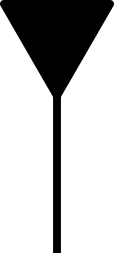
\includegraphics[width=.6cm]{clou_droit.png} & 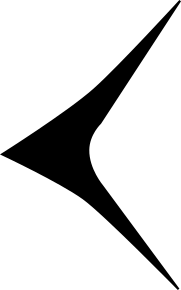
\includegraphics[width=.95cm]{chevron.png} \\\hline
Valeur & 1 & 10 \\
\end{tabular}
\end{center}

Ils utilisent un système sexagésimale (base $60$) et une numération de position. Suivant la place qu'occupe le symbole, celui-ci correspond soit à une unité, soit à une soixantaine ($60$), soit à une soixantaine de soixantaines ($60\times60=3\,600$). On utilise encore aujourd'hui un système sexagésimale pour les unités de temps et des mesures d'angles.\\

Exemples :
\begin{center}
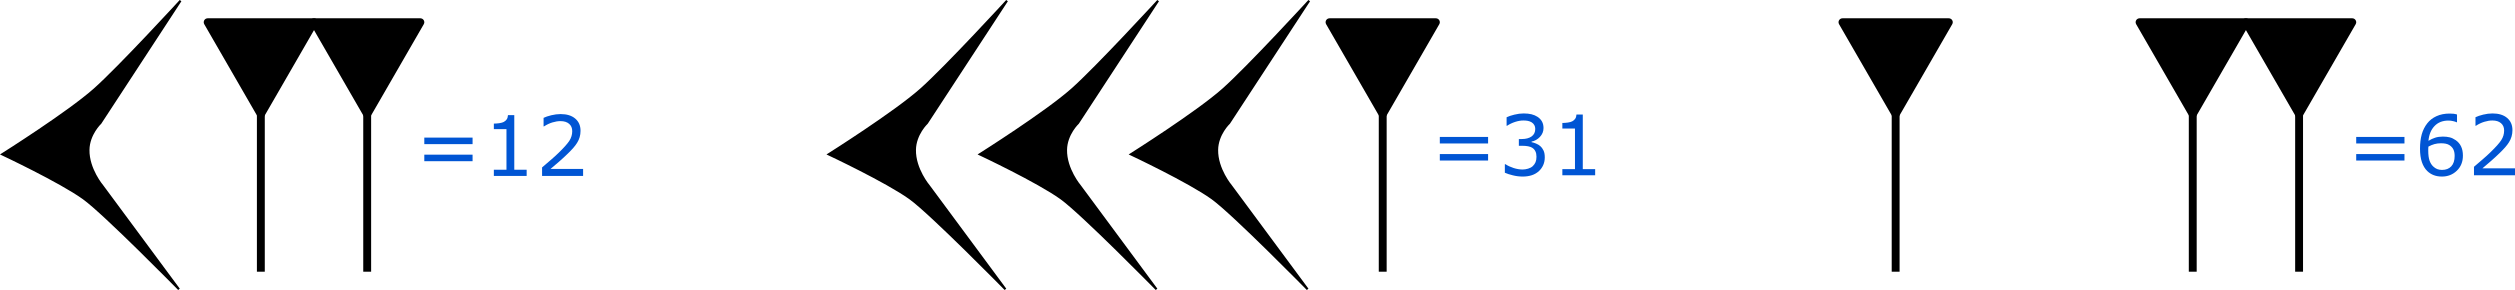
\includegraphics[width=9cm]{exemple_babylonian.png}
\end{center}
\end{His}

\subsection{La numération Égyptienne}

\begin{His}
Au \RNum{3}e millénaire avant J.C., en Egypte, les scribes écrivent les nombres sur des papyrus sous forme de hiéroglyphes. Les égyptiens utilisent un système de numération basé sur le principe additif. Les égyptiens peuvent écrire des nombres entiers jusqu'à $1\,000\,000$. Ils écrivent aussi des nombres décimaux et des fractions.

\newcommand{\egmil}[1]{\multido{\i=1+1}{#1}{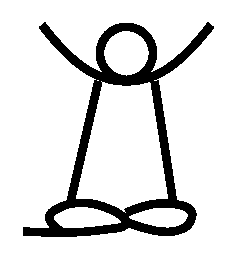
\includegraphics[scale=.1]{egyptian/egypt_person.eps}\hspace{0.5mm}}}
\newcommand{\eghuntho}[1]{\multido{\i=1+1}{#1}{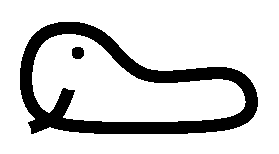
\includegraphics[scale=.1]{egyptian/egypt_fish.eps}\hspace{0.5mm}}}
\newcommand{\egtentho}[1]{\multido{\i=1+1}{#1}{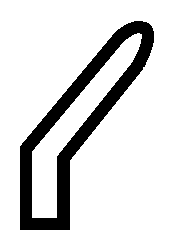
\includegraphics[scale=.1]{egyptian/egypt_finger.eps}\hspace{0.5mm}}}
\newcommand{\egtho}[1]{\multido{\i=1+1}{#1}{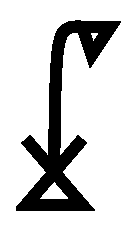
\includegraphics[scale=.1]{egyptian/egypt_lotus.eps}\hspace{0.5mm}}}
\newcommand{\eghun}[1]{\multido{\i=1+1}{#1}{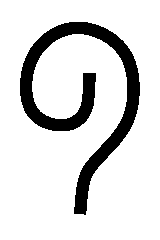
\includegraphics[scale=.1]{egyptian/egypt_scroll.eps}\hspace{0.5mm}}}
\newcommand{\egten}[1]{\multido{\i=1+1}{#1}{
\includegraphics[scale=.1]{egyptian/egypt_heel.eps}\hspace{0.5mm}}}
\newcommand{\egone}[1]{\multido{\i=1+1}{#1}{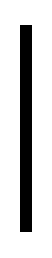
\includegraphics[scale=.1]{egyptian/egypt_stroke.eps}\hspace{0.5mm}}}
\newcommand{\egyptify}[7]{
 \multido{\i=1+1}{#1}{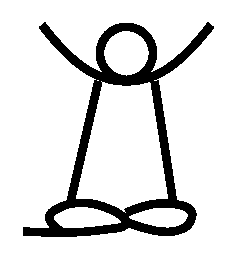
\includegraphics[scale=.1]{egyptian/egypt_person.eps}\hspace{0.5mm}}
 \multido{\i=1+1}{#2}{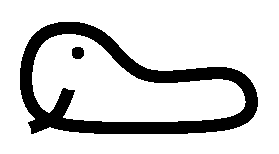
\includegraphics[scale=.1]{egyptian/egypt_fish.eps}\hspace{0.5mm}}
 \multido{\i=1+1}{#3}{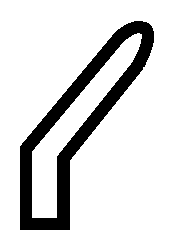
\includegraphics[scale=.1]{egyptian/egypt_finger.eps}\hspace{0.5mm}}
 \multido{\i=1+1}{#4}{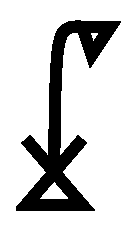
\includegraphics[scale=.1]{egyptian/egypt_lotus.eps}\hspace{0.5mm}}
 \multido{\i=1+1}{#5}{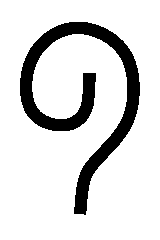
\includegraphics[scale=.1]{egyptian/egypt_scroll.eps}\hspace{0.5mm}}
 \multido{\i=1+1}{#6}{
\includegraphics[scale=.1]{egyptian/egypt_heel.eps}\hspace{0.5mm}}
 \multido{\i=1+1}{#7}{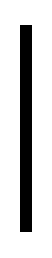
\includegraphics[scale=.1]{egyptian/egypt_stroke.eps}\hspace{0.5mm}}
 \hspace{.5mm}
}

\begin{center}
\begin{tabular}[t]{c|c|c|c|c|c|c}
\egmil{1}&\eghuntho{1}&\egtentho{1}&\egtho{1}&\eghun{1}&\egten{1}&\egone{1}\\
\hline
1,000,000&100,000&10,000&1,000&100&10&1\\
\end{tabular}\\
\end{center}

Exemple :

\begin{center}
\egyptify{5}{8}{6}{7}{9}{3}{4}$=5\,867\,934$
\end{center}
\end{His}

\subsection{La numération Maya}

\begin{His}
Dans leur étude des astres, les mayas se servent des nombres pour calculer le temps. Ce sont les inventeurs du calendrier.

 Leur système de numération datant du \RNum{5}e siècle après J.C. suit le principe de position dans la base vigésimale (base $20$). Celui-ci trouve ses origines avec nos $10$ doigts et $10$ orteils !  
 
 Les symboles employés (les glyphes) représentent les nombres jusqu'à $19$, empilés sur différents niveaux. Chaque niveau correspond à un nombre de paquets de $20$ puis de $20\times20=400$ puis de $20\times20\times20=8\,000$...
 
Les mayas utilisent le zéro qu'ils représentent par un coquillage.

\begin{center}
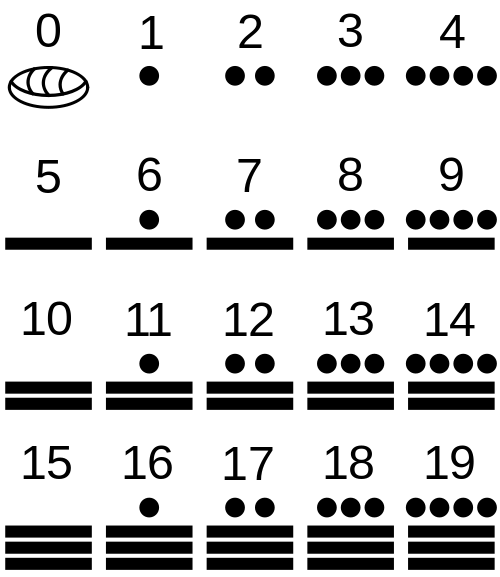
\includegraphics[width=8cm]{maya_numerals.png}
\end{center}

Exemple : $379=18\times20+19$
\begin{center}
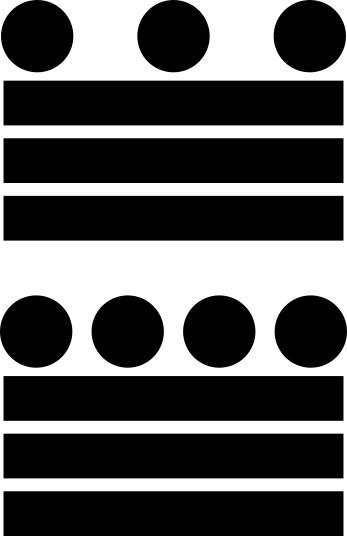
\includegraphics[width=1cm]{maya_exemple.png}
\end{center}
\end{His}

\subsection{La numération Romaine}

\begin{His}
Les grecs et les romains ont inventé des systèmes de numération alphabétiques très peu adaptés aux calculs.

Le système romain est composé de symboles notés côte à côte selon le principe additif et combine les bases $5$ et $10$.

Les plus anciens sont les signes \RNum{1}, \RNum{5}, et \RNum{10} qui dérivent directement de la pratique de l'entaille.

\begin{center}
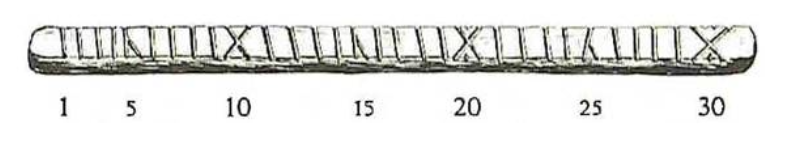
\includegraphics[width=8cm]{roman.png}
\end{center}

\begin{center}
\RNum{1}$=1$\hspace{.5cm}\RNum{2}$=2$\hspace{.5cm}\RNum{3}$=3$\hspace{.5cm}\RNum{4}$=4$\hspace{.5cm}\RNum{5}$=5$\\
\RNum{6}$=6$\hspace{.5cm}\RNum{7}$=7$\hspace{.5cm}\RNum{8}$=8$\hspace{.5cm}\RNum{9}$=9$\hspace{.5cm}\RNum{10}$=10$\\
\RNum{20}$=20$\hspace{.5cm}\RNum{50}$=50$\hspace{.5cm}\RNum{100}$=100$\hspace{.5cm}\RNum{500}$=500$\hspace{.5cm}\RNum{1000}$=1000$
\end{center}

Exemple :
\begin{center}
\RNum{6963}$=6\,963$
\end{center}
\end{His}

\subsection{L'histoire de nos chiffres}

\begin{His}
Nos chiffres de "$1$" à "$9$" que nous appelons à tort "chiffres arabes", viennent en réalité des Indes. Leurs "ancêtres" les plus anciens apparaissent dans des inscriptions des grottes de Nana Ghât datant du \RNum{2}e siècle avant J.C.

Au \RNum{5}e siècle de notre ère, en Inde, les savants ont l'idée ingénieuse de marier le principe de position, les neuf symboles et les zéro en tant que nombre à part entière représentant une quantité qui n'existe pas.

\begin{center}

\includegraphics[width=10cm]{indian1.png}\\
\textbf{Numération indienne}
\end{center}

Au \RNum{8}e siècle après J.C., alors que l'islam s'étend sur une partie de l'Afrique et de l'Asie, les califes de Bagdad font traduire les œuvres majeurs des peuples sur lesquels ils règnent.

Parmi elles se trouve l'œuvre de Brahmagupta, un mathématicien indien. Sa numération à dix chiffres est si ingénieuse que les marchands arabes l'adoptent immédiatement.

\begin{center}

\includegraphics[width=10cm]{indian2.png}\\
\textbf{Numération arabe}
\end{center}
\end{His}

\begin{His}
Au \RNum{9}e siècle, les chiffres arabes sont décrits dans un ouvrage du mathématicien et astronome Muhammad ibn Musa el-Khwarizmi ($790-850$) qui, traduit en latin, les diffuse en Espagne.\\

Gerbert d'Aurillac ($945-1003$) qui deviendra pape en $999$, est passionné par les mathématiques. Il rédige deux traités, l'un sur la multiplication, l'autre sur la division. Il initiera pour la première fois l'occident chrétien aux chiffres "indo-arabes" mais il ne retient ni la numération de position ni le zéro. 

\begin{center}

\includegraphics[width=10cm]{indian3.png}\\
\textbf{Numération hispano-arabe}
\end{center}

Au \RNum{13}e siècle, le mathématicien italien Léonard de Pise ($1175-1250$), dit Fibonacci publia, en $1202$, le \textit{Liber Abaci} (le livre du calcul), un traité sur les calculs et la comptabilité fondée sur le calcul décimal.\\

Au \RNum{15}e siècle, avec l'expansion de l'imprimerie, les chiffres ont été légèrement déformés pour donner une forme semblable à la forme actuelle. 

\begin{center}
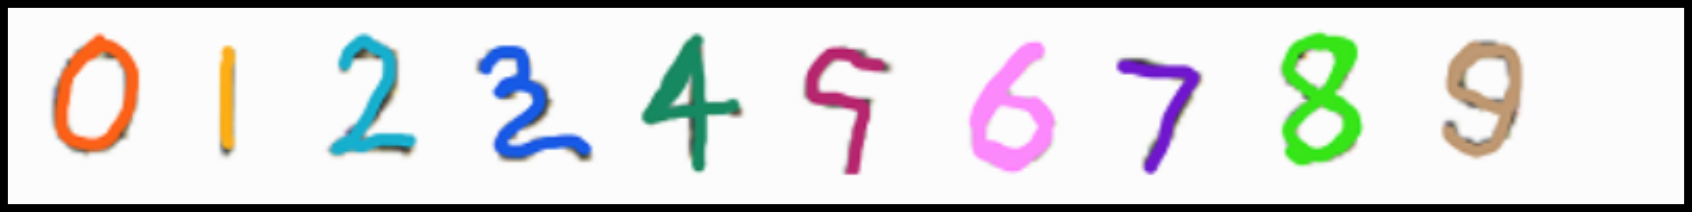
\includegraphics[width=10cm]{indian4.png}\\
\textbf{Numération italienne}
\end{center}
\end{His}

\section{Nombres entiers}

\begin{Def}
Un \textbf{nombre entier} est un nombre qui peut s'écrire \textbf{sans virgule}
\end{Def}

\begin{Rqs}
\begin{itemize}
\item $0$, $1$, $2$, $3$, $4$, $5$, $6$, $7$, $8$ et $9$ sont les dix \textbf{chiffres} qui permettent d'écrire tous les nombres entiers.
\item Pour pouvoir lire les grands nombres entiers facilement, on regroupe les chiffres par groupe de 3 : $345\,202$
\end{itemize}
\end{Rqs}

\begin{Reg}
Règles orthographiques pour l'écriture des nombres :
\begin{itemize}
    \item Un trait d'union entre chaque mot.
    \item Les mots servant à écrire les nombres sont tous invariable sauf :
    \begin{itemize}
        \item Au pluriel million et milliard prennent un 's'.
        \item Au pluriel cent et vingt prennent un 's' lorsqu'ils ne sont pas suivi par un autre nombre.
    \end{itemize}
\end{itemize}
\end{Reg}

\begin{Ex}
\begin{itemize}
\item $895$ s'écrit : 'huit-cent-quatre-vingt-quinze'
\item $1\,200$ s'écrit : 'mille-deux-cents'
\item $1\,230$ s'écrit : 'mille-deux-cent-trente'
\item $1\,280$ s'écrit : 'mille-deux-cent-quatre-vingts'
\item $1\,285$ s'écrit : 'mille-deux-cent-quatre-vingt-cinq'
\end{itemize}
\end{Ex}

\section{Position d'un chiffre dans un nombre}

\begin{Def}
\begin{itemize}
\item Notre système numérique est un \textbf{système décimal} (numération décimale).
\item Chaque \textbf{chiffre} à une valeur en fonction de sa \textbf{position} dans le nombre (numération de position)
\end{itemize}
\end{Def}

\begin{Ex}
Un million = $1\,000\,000$ unités
\end{Ex}

\begin{Voc}
Chaque position (rang) possède un nom spécifique : unité, dizaine, centaines....
    
\begin{center}
    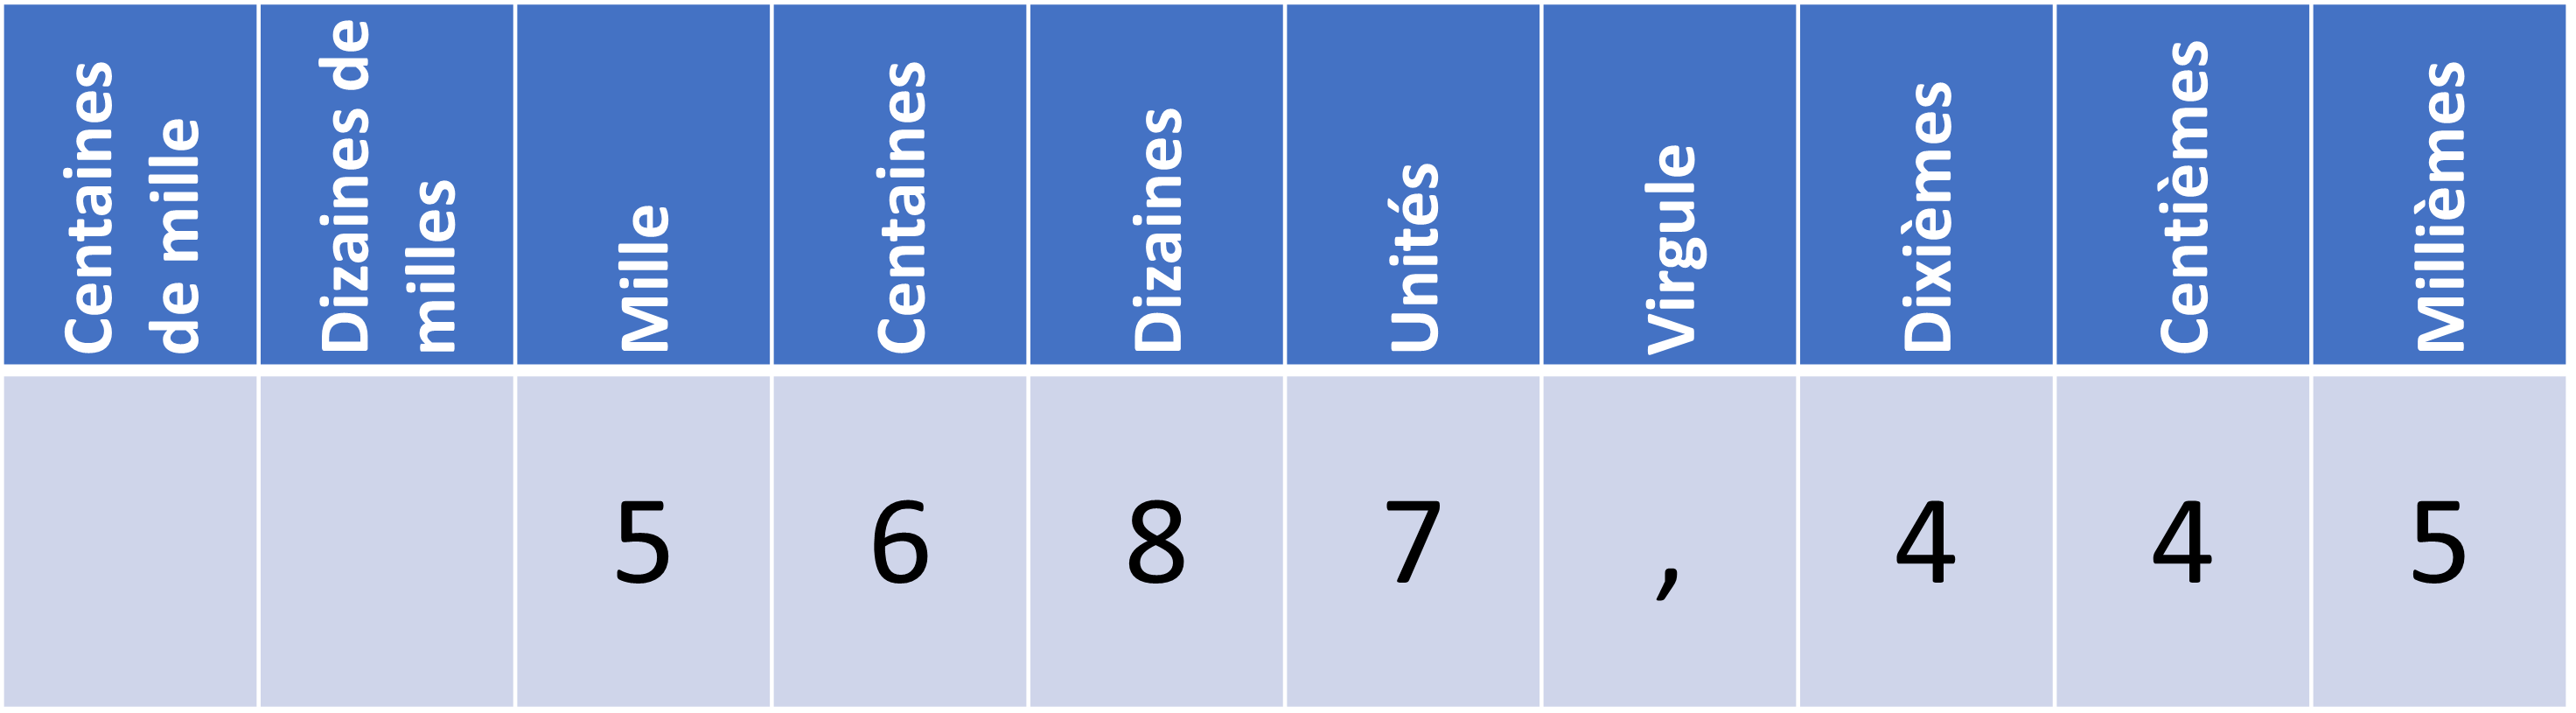
\includegraphics[width=13cm]{tableau_position.png}
\end{center}
\end{Voc}

\begin{Mt}
Décomposition de $437\,640\,881$ :
\begin{itemize}
\item Décomposition 1 : 
\[437\,000\,000+640\,000+881\]
\item Décomposition 2 :
\[(437\times1\,000\,000)+(640\times 1\,000)+(881\times1)\]
\item Décomposition 3 :
\[400\,000\,000+30\,000\,000+7\,000\,000+600\,000+40\,000+800+80+1\]
\item Décomposition 4 :
\[4\times100\,000\,000+3\times10\,000\,000+7\times1\,000\,000+6\times100\,000+4\times10\,000+8\times100+8\times10+1\times1\]
\end{itemize}
\end{Mt}

\section{Comparer des nombres entiers}

\begin{Def}
\textbf{Comparer} deux nombres, c'est trouver le \textbf{plus grand} (ou le \textbf{plus petit}) ou dire s'ils sont \textbf{égaux}.

On utilise les \textbf{symboles de comparaison} :
\begin{center}
est supérieur à ($>$) \hspace{1cm} est inférieur à ($<$) \hspace{1cm} est égal à ($=$)
\end{center}
\end{Def}

\begin{Ex}
$29\,874\,492$ est plus grand que $27\,514\,420$ donc $29\,874\,492>27\,514\,420$.
\end{Ex}

% \begin{ExOApp}[]
% Comparer les nombres suivants :

% \[567 \hspace{.5cm} 455\]
% \[91\,456\,022 \hspace{.5cm} 83\,427\,923\]
% \end{ExOApp} 

\begin{Def}
\begin{itemize}
\item Ranger des nombres dans \textbf{l'ordre croissant} signifie les ranger \textbf{du plus petit au plus grand}.
\item Ranger des nombres dans \textbf{l'ordre décroissant} signifie les ranger \textbf{du plus grand au plus petit}.
\end{itemize}
\end{Def}

% \begin{ExOApp}[]
% \begin{enumerate}
% \item Mettre les nombres suivants dans l'ordre croissant.

% \[93\,692 \hspace{.5cm} 83\,321 \hspace{.5cm} 44\,512 \hspace{.5cm} 65\,173\]
% \item Mettre les nombres suivants dans l'ordre décroissant.

% \[7\,096 \hspace{.5cm} 8\,623 \hspace{.5cm} 56\,393 \hspace{.5cm} 13\,582\]
% \end{enumerate}
% \end{ExOApp}

\section{Encadrer un nombre entier}

\begin{Def}
\textbf{Encadrer} un nombre, c'est trouver un nombre plus petit et un nombre plus grand.

La \textbf{précision de l'encadrement} est la \textbf{différence} entre les deux nombres trouvés.
\end{Def}

\begin{Ex}
Encadrement du nombre $56$ :
 \begin{itemize}
\item Encadrement à la dizaine : \(50 < 56< 60\)

\item Encadrement au centième : \(0 < 56< 100\)
 \end{itemize}
\end{Ex}

% \begin{ExOApp}[]
% Encadrer le nombre $33\,935$ à la \textbf{centaine} près.
% \end{ExOApp}

\section{Nombres entiers et demi-droite graduée}

\begin{Def}
Une \textbf{demi-droite graduée} est une \textbf{demi-droite} sur laquelle on a reporté une \textbf{unité de longueur} régulièrement à partir de son \textbf{origine}.

Sur une demi-droite graduée, \textbf{un point} est repéré par \textbf{un nombre}, son \textbf{abscisse}.

Si un point $A$ a pour abscisse $6$, on note : $A(6)$.

L'origine est repérée par le nombre $0$.

\begin{center}
\begin{tikzpicture}[line cap=round,line join=round,>=triangle 45,x=1.0cm,y=1.0cm]
\begin{axis}[
x=1.0cm,y=1.0cm,
axis lines=middle,
xmin=-0.1994343408245771,
xmax=9.60761325487766,
ymin=-0.4707007586686898,
ymax=0.44760621908013903,
xtick={-0.0,1.0,...,9.0},
ytick={-0.0,1.0,...,0.0},]
\clip(-0.1994343408245771,-0.4707007586686898) rectangle (9.60761325487766,0.44760621908013903);
\draw [->,line width=2.pt] (0.,0.) -- (9.619386421259055,0.);
\begin{scriptsize}
\draw [fill=xdxdff] (6.,0.) circle (2.5pt);
\draw[color=xdxdff] (6.087436506840482,0.21802947464293182) node {$A$};
\end{scriptsize}
\end{axis}
\end{tikzpicture}
\end{center}

\end{Def}

% \begin{ExOApp}[]
% Sur la demi-droite ci-dessous :

% \begin{enumerate}
% \item Donner les abscisses des points A, B et C.\\
% \[A(............)\hspace{1cm}B(............)\hspace{1cm}C(............)\]
% \item Placer le point D(35).
% \end{enumerate} 

% \begin{center}
    % 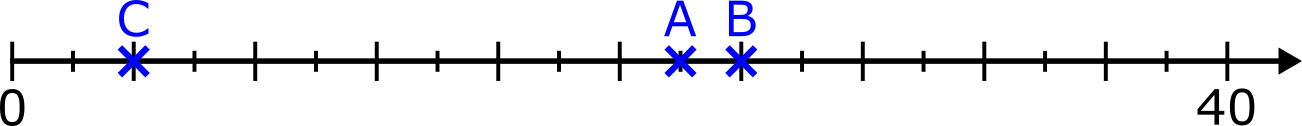
\includegraphics[width=12cm]{demi_droite.png}
% \end{center}
% \end{ExOApp}

% \section{Les savoir-faire du parcours}

% \begin{CpsCol}
% \begin{itemize}
% \item Savoir écrire un nombre entier en lettres.
% \item Savoir écrire un nombre entier en chiffres.
% \item Savoir déterminer la valeur d'un chiffre selon sa position.
% \item Savoir déterminer un nombre de ... dans un nombre entier.
% \item Savoir décomposer un nombre entier.
% \item Savoir comparer des nombres entiers.
% \item Savoir encadrer un nombre entier.
% \item Savoir repérer un nombre entier sur une demi-droite graduée.
% \item Savoir placer un nombre sur une demi-droite graduée.
% \end{itemize}
% \end{CpsCol}

% \end{document}

\end{pageCours} 
